% --- IMPORTS ---
\documentclass[leqno]{article}
\usepackage{graphicx}
\usepackage{dsfont}
\usepackage{mathtools}
\usepackage{amssymb}
\usepackage{amsmath}
\usepackage{amsthm}
\usepackage{float}
\usepackage{ragged2e}
\usepackage{tensor}
\usepackage{fancyhdr}
\usepackage{empheq}
\usepackage[most]{tcolorbox}
\usepackage{enumitem}
\usepackage{dirtytalk}
\usepackage{marginnote}
\usepackage{microtype}
\usepackage[
  a4paper,
  left=0.8in,
  right=1in,
  top=1in,
  bottom=0.5in,
  headheight=14pt,
  headsep=0.4in
]{geometry}
\setlength{\parindent}{0cm}
% --- TikZ Packages ---
\usepackage{pgfplots}
\pgfplotsset{compat=1.18}
\usepgfplotslibrary{fillbetween, polar}
\usetikzlibrary{calc, positioning}
\usetikzlibrary{angles, quotes}
\usetikzlibrary{arrows.meta}
\usetikzlibrary{decorations.pathreplacing, decorations.markings}
\usetikzlibrary{patterns}
\usetikzlibrary{intersections}
% --- URL Packages ---
\usepackage[colorlinks=true,linkcolor=red,citecolor=magenta,urlcolor=black]{hyperref}%
\urlstyle{same}
% --- END OF IMPORTS ---

% --- CUSTOM COMMANDS ---
\RenewDocumentCommand{\marks}{o m}{%
  \IfValueTF{#1}%
    {\marginnote{\raggedright\textbf{[#2]}}[#1]}%
    {\marginnote{\raggedright\textbf{[#2]}}}%
}
\newcommand{\vspacerule}[2]{%
  \par\vspace*{#1}%
  \noindent\hrulefill\par
  \vspace*{#2}%
}
\definecolor{scarlet}{RGB}{205, 40, 75}
\newcommand{\questionitem}{%
  \item\phantomsection
  \addcontentsline{toc}{section}{Question \number\value{enumi}}%
}
\renewcommand{\contentsname}{Questions}
\newcommand{\timingbox}[4]{%
  \vspace*{20pt}
  \noindent\begin{tcolorbox}[
    enhanced, sharp corners,
    width=0.8\textwidth,
    colback=white, colframe=white, boxrule=0pt,
    borderline west={3pt}{0pt}{scarlet},
    left=20pt, right=20pt, top=12pt, bottom=12pt,
    before skip=0pt, after skip=0pt
  ]
  {\LARGE\bfseries #1}\\[8pt]
  {\normalsize Total Marks: #2 }\\[6pt]
  {\normalsize  #3\\[6pt]
  Complete in \textbf{#4}}
  \end{tcolorbox}
  \vspace*{20pt}%
}
% --- END OF CUSTOM COMMANDS ---

% --- HEADER CONFIG ---
\pagestyle{fancy}
\fancyhead{}
\fancyfoot{}
\renewcommand{\headrulewidth}{0.9pt}
\lhead{Work-Energy Principle}
\chead{}
\rhead{\href{https://danieljsmith.org}{danieljsmith.org}}
% --- END OF HEADER CONFIG ---

\begin{document}
\vspace*{20pt}
\tableofcontents
\newpage
\begin{enumerate}[
  label=\textbf{\arabic*.},
  leftmargin=*,
  topsep=0pt,
  partopsep=0pt,
  parsep=0pt
]


% ---- Question 1 ----
\questionitem
% [Source: _QBT__Work_Energy_Principle, Q1]

\begin{figure}[H]
    \centering
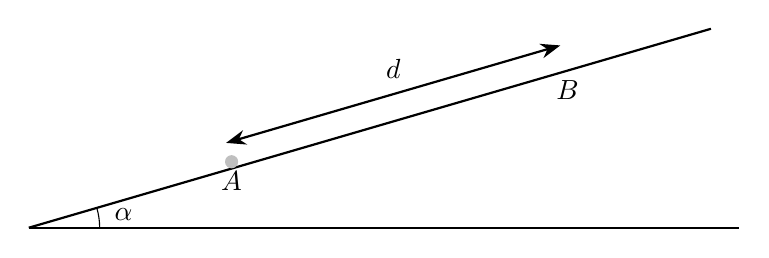
\begin{tikzpicture}[scale=0.95]
\def\run{24}
\def\rise{7}
\def\scaleFactor{0.38}
\def\dimOffset{0.35}
\def\particleRadius{2.5pt}
\pgfmathsetmacro{\ang}{atan(\rise/\run)}
\pgfmathsetmacro{\slopeLen}{\scaleFactor*sqrt(\run*\run+\rise*\rise)}

\coordinate (base) at (0,0);
\coordinate (top) at (\ang:\slopeLen);
\coordinate (Aplane) at ($(base)!0.30!(top)$);
\coordinate (B) at ($(base)!0.79!(top)$);
\coordinate (A) at ($(Aplane)+({90+\ang}:\particleRadius)$);
\coordinate (horiz) at (\slopeLen,0);
\coordinate (dA) at ($(Aplane)+({90+\ang}:\dimOffset)$);
\coordinate (dB) at ($(B)+({90+\ang}:\dimOffset)$);

\draw[thick, black] (base) -- (top);
\draw[thick, black] (base) -- (horiz);
\fill[gray!50, yshift=5pt] (A) circle (\particleRadius);

\node[below] at (A) {$A$};
\node[below] at (B) {$B$};
\draw[{Stealth[length=2.5mm]}-{Stealth[length=2.5mm]}, thick, black]
  (dA) -- node[midway, above=2pt] {$d$} (dB);

\pic["$\alpha$", draw, angle radius=9mm, angle eccentricity=1.35] {angle=horiz--base--top};
\end{tikzpicture}
\end{figure}


A particle of mass $m$ is at a point $A$ on a rough plane. \\

The plane is inclined at an angle $\alpha$ to the horizontal, where $\sin\alpha=\dfrac{7}{25}$. \\

The coefficient of friction between the particle and the plane is $\dfrac{1}{3}$. \\

The points $A$ and $B$ lie on a line of greatest slope of the plane, with $B$ above $A$, and $AB=d$, as shown in the diagram. \\

\begin{enumerate}[label=\textbf{(\alph*)}]
  \item Show that the work done against friction as the particle moves from $A$ to $B$ is
  \[
  \dfrac{8}{25}mgd
  \]
  \marks[-20pt]{3}
  \item The particle is projected up the line of greatest slope from $A$ towards $B$ with speed $\sqrt{gd}$. \\
  Use the work-energy principle to determine whether the particle reaches $B$. If it does not, find how far it travels from $A$ before coming instantaneously to rest. \marks{4} \\
\end{enumerate}
\newpage
% ---- Question 2 ----
\questionitem
% [Source: _QBT__Work_Energy_Principle, Q2]

A plane is inclined to the horizontal at an angle $\alpha$, where $\tan\alpha=\dfrac{5}{12}$. \\

A point $B$ lies on the plane such that $AB=39\text{ m}$. \\

A particle $P$ is projected with speed $21\text{ m s}^{-1}$ from $A$, up a line of greatest slope of the plane. \\

In an initial model, the plane is modelled as being smooth and air resistance is modelled as being negligible. \\

Using this model and the principle of conservation of mechanical energy, \\

\begin{enumerate}[label=\textbf{(\alph*)}]
  \item find the speed of $P$ when it reaches $B$. \marks{4} \\
\end{enumerate}

In a refined model, the plane is now modelled as being rough, with the coefficient of friction between $P$ and the plane being $\dfrac{1}{3}$. \\

Air resistance is still modelled as being negligible. \\

Using this refined model and the work-energy principle, \\

\begin{enumerate}[label=\textbf{(\alph*)}, resume]
  \item determine whether $P$ reaches $B$. If it does not, find the distance travelled by $P$ up the plane from $A$ before it comes instantaneously to rest. \marks{8} \\
\end{enumerate}

\newpage

% ---- Question 3 ----
\questionitem
% [Source: _QBT__Work_Energy_Principle, Q3]

A sledge of mass $40\,\mathrm{kg}$ is pulled up a rough slope inclined at $10^\circ$ to the horizontal. \\

The coefficient of friction between the sledge and the slope is $0.25$. \\

The sledge is at rest when a rope starts to pull it. \\

The tension in the rope is $220\,\mathrm{N}$ and the rope makes an angle of $15^\circ$ above the slope. \\

After the sledge has moved $5$ metres up the slope, the rope breaks. \\

\begin{enumerate}[label=\textbf{(\alph*)}]
  \item Use an energy method to find the maximum speed of the sledge. \marks{4} \\
  \item Use an energy method to find the total distance the sledge moves up the slope before coming to rest. \marks{2} \\
  \item A student claims that in reality the sledge is unlikely to move more than $6.8$ metres up the slope in total. Comment on the validity of this claim. \marks{2} \\
\end{enumerate}

\newpage

% ---- Question 4 ----
\questionitem
% [Source: _QBT__Work_Energy_Principle, Q4]


\begin{figure}[H]
\centering
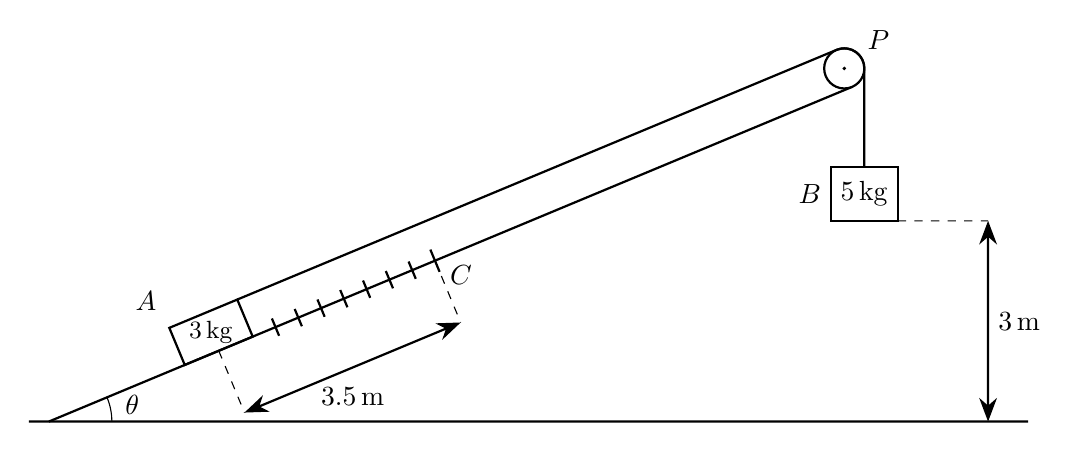
\begin{tikzpicture}[scale=0.85]
\def\run{12}
\def\rise{5}
\pgfmathsetmacro{\ang}{atan(\rise/\run)}
\pgfmathsetmacro{\slopeLen}{veclen(\run,\rise)}

\def\rad{0.30}
\def\bw{1.1}
\def\bh{0.60}
\def\hbw{1.0}
\def\hbh{0.8}

\def\AposFromBase{2.75}
\def\roughLen{3.5}
\def\Bclearance{3.0}
\pgfmathsetmacro{\halfBw}{0.5*\bw}

\coordinate (O) at (0,0);
\coordinate (X) at (2,0);
\coordinate (T) at (\run,\rise);
\pgfmathsetmacro{\afrac}{\AposFromBase/\slopeLen}
\coordinate (Apos) at ($(O)!\afrac!(T)$);
\coordinate (Aleft) at ($(Apos)+(\ang+180:\halfBw)$);
\coordinate (Afront) at ($(Apos)+(\ang:\halfBw)$);
\coordinate (C) at ($(Apos)+(\ang:\roughLen)$);

\coordinate (Pc) at ($(T)+(\ang+90:\rad)$);
\coordinate (Sleft) at ($(Pc)+(\ang+90:\rad)$);
\coordinate (Sright) at ($(Pc)+(0:\rad)$);

\pgfmathsetmacro{\drop}{\rise + \rad*cos(\ang) - (\Bclearance+\hbh)}
\coordinate (Btop) at ($(Sright)+(0,-\drop)$);
\coordinate (BbottomRight) at ($(Btop)+({\hbw/2},{-\hbh})$);
\coordinate (DimTop) at ($(BbottomRight)+(1.35,0)$);
\coordinate (DimBot) at ($(DimTop)+(0,-\Bclearance)$);

\draw[thick] (-0.3,0) -- ($(DimBot)+(0.6,0)$);
\draw[thick] (O) -- (T);

\pic[draw, "$\theta$", angle radius=8mm, angle eccentricity=1.35]
  {angle=X--O--T};

\foreach \i in {1,...,7} {
  \pgfmathsetmacro{\s}{\halfBw + \i*(\roughLen-\halfBw)/8}
  \coordinate (R\i) at ($(Apos)+(\ang:\s)$);
  \draw[thick] ($(R\i)+(\ang+90:0.14)$) -- ($(R\i)+(\ang-90:0.14)$);
}
\draw[thick] ($(C)+(\ang+90:0.18)$) -- ($(C)+(\ang-90:0.18)$);

\begin{scope}[shift={(Aleft)}, rotate=\ang]
  \draw[thick] (0,0) rectangle (\bw,\bh);
  \coordinate (Aattach) at (\bw,\bh);
  \coordinate (AupperLeft) at (0,\bh);
  \node[font=\small] at ({0.5*\bw},{0.5*\bh}) {$3\,\mathrm{kg}$};
\end{scope}

\fill[white] (Pc) circle (\rad);
\draw[thick] (Pc) circle (\rad);
\fill (Pc) circle (0.8pt);

\draw[thick]
  ($(Btop)+({-\hbw/2},0)$) rectangle ($(Btop)+({\hbw/2},{-\hbh})$);
\node at ($(Btop)+(0,{-0.5*\hbh})$) {$5\,\mathrm{kg}$};

\draw[thick] (Aattach) -- (Sleft);
\draw[thick] (Sleft) arc[start angle={\ang+90}, end angle=0, radius=\rad];
\draw[thick] (Sright) -- (Btop);

\node[above left] at ($(AupperLeft)+(\ang+90:0.12)$) {$A$};
\node[fill=white, inner sep=1pt, anchor=south east]
  at ($(C)+(\ang+90:-0.6)+(\ang:0.4)$) {$C$};
\node[anchor=west, inner sep=1pt]
  at ($(Pc)+(55:0.52)$) {$P$};
\node[left] at ($(Btop)+({-\hbw/2},{-0.5*\hbh})$) {$B$};


\coordinate (DimA) at ($(Apos)+(\ang-90:1.00)$);
\coordinate (DimC) at ($(C)+(\ang-90:1.00)$);
\draw[dashed] (Apos) -- (DimA);
\draw[dashed] (C) -- (DimC);
\draw[thick, {Stealth[length=3mm]}-{Stealth[length=3mm]}]
  (DimA) -- (DimC)
  node[midway, below=6pt, fill=white, inner sep=1pt] {$3.5\,\mathrm{m}$};

\draw[dashed] (BbottomRight) -- (DimTop);
\draw[thick, {Stealth[length=3mm]}-{Stealth[length=3mm]}]
  (DimBot) -- (DimTop)
  node[midway,right] {$3\,\mathrm{m}$};
\end{tikzpicture}
\end{figure}
\vspace*{10pt}

Two blocks, $A$ and $B$, of masses $3\,\mathrm{kg}$ and $5\,\mathrm{kg}$ respectively are attached to the ends of a light inextensible string. \\

Initially $A$ is held on a fixed plane. The plane is inclined to horizontal ground at an angle $\theta$, where $\tan\theta=\dfrac{5}{12}$. \\

The string passes over a small smooth light pulley $P$ that is fixed at the top of the plane. The part of the string from $A$ to $P$ is parallel to a line of greatest slope of the plane. \\

The section of the plane from the initial position of $A$ to a point $C$, $3.5\,\mathrm{m}$ up the plane, is rough. The section from $C$ to $P$ is smooth. \\

Block $B$ hangs freely below $P$ at a distance of $3\,\mathrm{m}$ above the ground, as shown in the diagram. The coefficient of friction between $A$ and the rough part of the plane is $\mu$. Block $A$ is released from rest with the string taut. \\

By modelling the blocks as particles, \\

\begin{enumerate}[label=\textbf{(\alph*)}]
  \item find the potential energy lost by the whole system as a result of $B$ falling $3\,\mathrm{m}$. \marks{3} \\
\end{enumerate}

Given that the speed of $B$ at the instant it hits the ground is $4.8\,\mathrm{m\,s^{-1}}$ and ignoring air resistance, \\

\begin{enumerate}[label=\textbf{(\alph*)}, resume]
  \item use the work-energy principle to find the value of $\mu$. \marks{6} \\
\end{enumerate}

After $B$ hits the ground, $A$ continues to move up the plane, passes $C$ and does not reach the pulley in the subsequent motion. \\

Block $A$ comes to instantaneous rest after moving a total distance of $(3.5+d)\,\mathrm{m}$ from its point of release. \\

Ignoring air resistance, \\

\begin{enumerate}[label=\textbf{(\alph*)}, resume]
  \item use the work-energy principle to find the value of $d$. \marks{4} \\
\end{enumerate}

\newpage

% ---- Question 5 ----
\questionitem
% [Source: _QBT__Work_Energy_Principle, Q5]


A crate, of mass $10\,\mathrm{kg}$, is pulled up a rough plane inclined at $15^\circ$ to the horizontal. \\

The crate is attached to a light string. The string lies in the vertical plane of greatest slope and is inclined at $20^\circ$ above the plane. \\

The tension in the string is $80$ newtons. \\

As the crate moves a distance of $x$ metres up the plane, its speed increases from $1.5\,\mathrm{m\,s^{-1}}$ to $4.5\,\mathrm{m\,s^{-1}}$. \\

The coefficient of friction between the crate and the plane is $0.3$. \\

\begin{enumerate}[label=\textbf{(\alph*)}]
  \item By using an energy method, find $x$. \marks{6} \\
  \item Describe how the model could be refined to obtain a more realistic value of $x$ and use an energy argument to explain whether this would increase or decrease the value of $x$. \marks{2} \\
\end{enumerate}

\newpage

% ---- Question 6 ----
\questionitem
% [Source: _QBT__Work_Energy_Principle, Q6]

\begin{figure}[H]
    \centering
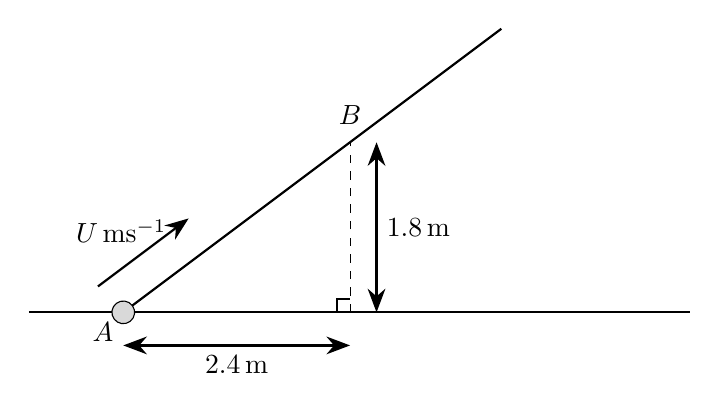
\begin{tikzpicture}[scale=1.2]
\def\horiz{2.4}
\def\rise{1.8}
\def\extra{2.0}
\def\groundleft{1.0}
\def\groundright{2.0}
\def\dimoff{0.35}
\def\voff{0.28}
\def\ra{0.14}
\def\particleRad{0.12}
\def\ustart{-0.05}
\def\uoffset{0.38}
\def\ulen{1.2}
\pgfmathsetmacro{\AB}{veclen(\horiz,\rise)}
\pgfmathsetmacro{\ang}{atan(\rise/\horiz)}
\pgfmathsetmacro{\mult}{1+\extra/\AB}
\pgfmathsetmacro{\groundend}{\horiz*\mult+\groundright}

\coordinate (A) at (0,0);
\coordinate (D) at (\horiz,0);
\coordinate (B) at (\horiz,\rise);
\coordinate (top) at ($(A)!\mult!(B)$);

\draw[thick, black] (-\groundleft,0) -- (\groundend,0);
\draw[thick, black] (A) -- (top);
\draw[dashed, black] (D) -- (B);

\draw[thick, black] ($(D)+(-\ra,0)$) -- ($(D)+(-\ra,\ra)$) -- ($(D)+(0,\ra)$);

\begin{scope}[shift={(A)}, rotate=\ang]
  \filldraw[fill=gray!30, draw=black] (0,0) circle (\particleRad);
  \draw[-{Stealth[length=3mm]}, thick, black] (\ustart,\uoffset) -- ++(\ulen,0)
    node[midway, above, xshift=-8pt] {$U\,\text{ms}^{-1}$};
\end{scope}

\draw[{Stealth[length=3mm]}-{Stealth[length=3mm]}, thick, black]
  ($(A)+(0,-\dimoff)$) -- ($(D)+(0,-\dimoff)$)
  node[midway, below] {$\horiz\,\text{m}$};

\draw[{Stealth[length=3mm]}-{Stealth[length=3mm]}, thick, black]
  ($(D)+(\voff,0)$) -- ($(B)+(\voff,0)$)
  node[midway, right] {$\rise\,\text{m}$};

\node[below left] at (A) {$A$};
\node[above, yshift=3pt] at (B) {$B$};
\end{tikzpicture}
\end{figure}


A rough loading ramp is fixed to horizontal ground. Point $A$ is the lower end of the ramp and point $B$ lies on the ramp above $A$, as shown in the diagram above. \\

The point vertically below $B$ is $2.4\,\text{m}$ horizontally from $A$, and $B$ is $1.8\,\text{m}$ above the ground. \\

A crate of mass $2.5\,\text{kg}$ is projected up the ramp from $A$ with speed $U\,\text{m s}^{-1}$ and first comes to instantaneous rest at $B$. \\

The coefficient of friction between the crate and the ramp is $\dfrac{1}{4}$. \\

The crate is modelled as a particle. \\

\begin{enumerate}[label=\textbf{(\alph*)}]
  \item Find the work done against friction as the crate moves from $A$ to $B$. \marks{3} \\
  \item Use the work-energy principle to find the value of $U$. \marks{4} \\
\end{enumerate}

After coming to instantaneous rest at $B$, the crate slides back down the ramp. \\

\begin{enumerate}[label=\textbf{(\alph*)}, resume]
  \item Use the work-energy principle to find the speed of the crate at the instant it returns to $A$. \marks{3} \\
\end{enumerate}

\newpage

% ---- Question 7 ----
\questionitem
% [Source: _QBT__Work_Energy_Principle, Q7]

\begin{figure}[H]
    \centering
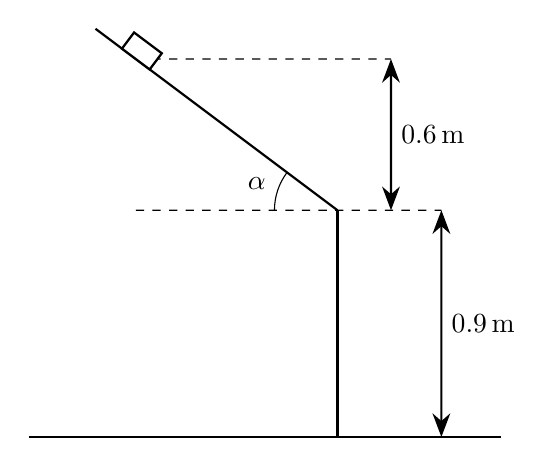
\begin{tikzpicture}[scale=0.8]
\pgfmathsetmacro{\ang}{asin(3/5)}
\pgfmathsetmacro{\roofang}{180-\ang}

\def\unit{4}
\pgfmathsetmacro{\eaveh}{0.9*\unit}
\pgfmathsetmacro{\rise}{0.6*\unit}
\pgfmathsetmacro{\roofdist}{\rise/sin(\ang)}
\pgfmathsetmacro{\rooflen}{\roofdist+0.8}

\def\boxw{0.55}
\def\boxh{0.32}
\def\dimsepA{0.85}
\def\dimsepB{1.65}

\coordinate (F) at (0,0);
\coordinate (E) at (0,\eaveh);
\coordinate (P) at ($(E)+(\roofang:\roofdist)$);
\coordinate (L) at ($(E)+(\roofang:\rooflen)$);
\coordinate (H) at (P|-E);

\coordinate (Vlo) at ($(E)+(\dimsepA,0)$);
\coordinate (Vhi) at ($(Vlo)+(0,\rise)$);
\coordinate (Wlo) at ($(F)+(\dimsepB,0)$);
\coordinate (Whi) at ($(Wlo)+(0,\eaveh)$);

\draw[thick] ($(F)+(-4.9,0)$) -- ($(F)+(2.6,0)$);
\draw[thick] (F) -- (E);
\draw[thick] (L) -- (E);

\draw[dashed] (P) -- (Vhi);
\draw[dashed] (H) -- (Whi);

\begin{scope}[shift={(P)}, rotate=\roofang]
  \draw[thick, fill=white] (-\boxw/2,0) rectangle (\boxw/2,-\boxh);
\end{scope}

\draw[{Stealth[length=3mm]}-{Stealth[length=3mm]}, thick] (Vlo) -- (Vhi)
  node[midway, right] {$0.6\,\mathrm{m}$};

\draw[{Stealth[length=3mm]}-{Stealth[length=3mm]}, thick] (Wlo) -- (Whi)
  node[midway, right] {$0.9\,\mathrm{m}$};

\path pic["$\alpha$", draw, angle radius=8mm, angle eccentricity=1.35]
  {angle=L--E--H};
\end{tikzpicture}
\end{figure}


A parcel of mass $m$ is held on a rough straight roof which is inclined at an angle $\alpha$ to the horizontal, where $\sin\alpha=\dfrac{3}{5}$. The parcel is released from rest at a point on the roof that is $0.6\,\mathrm{m}$ vertically above the eaves, as shown in the diagram above. The eaves are $0.9\,\mathrm{m}$ above the ground. The coefficient of friction between the parcel and the roof is $0.25$. \\

The parcel is modelled as a particle which, after leaving the roof, is assumed to move freely under gravity. \\

\begin{enumerate}[label=\textbf{(\alph*)}]
  \item Find, in terms of $m$ and $g$, the magnitude of the normal reaction on the parcel as it slides down the roof. \marks{2} \\
  \item Use the work-energy principle to find the speed of the parcel as it hits the ground. \marks{5} \\
\end{enumerate}

\newpage

% ---- Question 8 ----
\questionitem
% [Source: _QBT__Work_Energy_Principle, Q8]

A rough plane is inclined to the horizontal at an angle $\theta$, where $\tan\theta=\dfrac{5}{12}$. \\

A particle $P$ of mass $m$ is at rest at a point $O$ on the plane. \\

The coefficient of friction between $P$ and the plane is $\dfrac{1}{4}$. \\

The particle is projected up the plane with speed $4\sqrt{ag}$. \\

The particle moves up a line of greatest slope of the plane, comes to instantaneous rest, and then slides back down to $O$. \\

\begin{enumerate}[label=\textbf{(\alph*)}]
  \item Show that the magnitude of the frictional force acting on $P$ is
  \[
  \dfrac{3mg}{13}
  \]
  \marks[-20pt]{3}
\end{enumerate}
Air resistance is assumed to be negligible. \\

Using the work-energy principle, \\

\begin{enumerate}[label=\textbf{(\alph*)}, resume]
  \item find the speed of $P$ when it returns to $O$. \marks{5} \\
\end{enumerate}

\newpage

% ---- Question 9 ----
\questionitem
% [Source: _QBT__Work_Energy_Principle, Q9]
\begin{figure}[H]
    \centering
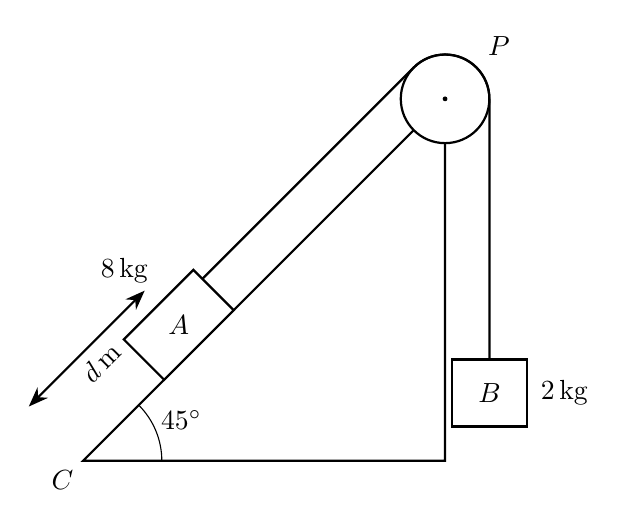
\begin{tikzpicture}[scale=1.25]
\def\ang{45}
\def\slopelen{5.2}
\def\pulrad{0.45}
\def\abw{1.0}
\def\abh{0.58}
\def\bbw{0.76}
\def\bbh{0.68}
\def\afrac{0.32}
\def\mdist{0.78}
\def\bdrop{2.65}
\pgfmathsetmacro{\run}{\slopelen*cos(\ang)}

\coordinate (C) at (0,0);
\coordinate (P) at (\ang:\slopelen);
\coordinate (R) at (\run,0);

\draw[thick] (C) -- (P) -- (R) -- cycle;

\pic["$45^\circ$", draw, angle radius=10mm, angle eccentricity=1.35]
  {angle=R--C--P};

\node[below left] at (C) {$C$};

\coordinate (Afoot) at ($(C)!\afrac!(P)$);
\begin{scope}[shift={(Afoot)}, rotate=\ang]
  \draw[thick, fill=white] (-\abw/2,0) rectangle (\abw/2,\abh);
  \coordinate (Acentre) at (0,\abh/2);
  \coordinate (Aattach) at (\abw/2,\pulrad);
  \node at (Acentre) {$A$};
\end{scope}
\node at ($(Acentre)+(\ang+90:0.78)$) {$8\,\mathrm{kg}$};

\coordinate (T1) at ($(P)+(\ang+90:\pulrad)$);
\coordinate (T2) at ($(P)+(0:\pulrad)$);

\draw[thick, fill=white] (P) circle (\pulrad);
\fill (P) circle (0.7pt);
\node[above right=1pt] at ($(P)+(45:\pulrad)$) {$P$};

\draw[thick] (Aattach) -- (T1);
\draw[thick] (T1) arc[start angle=\ang+90, end angle=0, radius=\pulrad];

\coordinate (Btop) at ($(T2)+(0,-\bdrop)$);
\coordinate (Bcentre) at ($(Btop)+(0,-\bbh/2)$);

\draw[thick, fill=white]
  ($(Btop)+(-\bbw/2,0)$) rectangle ($(Btop)+(\bbw/2,-\bbh)$);

\node at (Bcentre) {$B$};
\node[right=15pt] at (Bcentre) {$2\,\mathrm{kg}$};

\draw[thick] (T2) -- (Btop);

\coordinate (D0) at ($(C)+(\ang+90:\mdist)$);
\coordinate (D1) at ($(Afoot)+(\ang+90:\mdist)$);

\draw[{Stealth[length=2.5mm]}-{Stealth[length=2.5mm]}, thick]
  (D0) -- (D1) node[midway, sloped, below] {$d\,\mathrm{m}$};

\end{tikzpicture}
\end{figure}


One end of a rope is attached to a block $A$ of mass $8\,\mathrm{kg}$. The other end of the rope is attached to a second block $B$ of mass $2\,\mathrm{kg}$. Block $A$ is held at rest on a fixed rough ramp inclined at $45^\circ$ to the horizontal. The lower end of the ramp is $C$. The rope is taut and passes over a small smooth pulley $P$ which is fixed at the top of the ramp. The part of the rope from $A$ to $P$ is parallel to a line of greatest slope of the ramp. Block $A$ is initially $d\,\mathrm{m}$ from $C$, as shown in the diagram. \\

Block $B$ is more than $d\,\mathrm{m}$ below $P$. The blocks are released from rest and $A$ moves down the ramp towards $C$. \\

The coefficient of friction between $A$ and the ramp is $\dfrac{1}{4}$. \\

The blocks are modelled as particles, the rope is modelled as light and inextensible, and air resistance can be ignored. \\

\begin{enumerate}[label=\textbf{(\alph*)}]
  \item Determine, in terms of $g$ and $d$, the work done against friction as $A$ moves $d\,\mathrm{m}$ down the ramp. \marks{3} \\
  \item Given that the speed of $A$ immediately before it reaches $C$ is $2.1\,\mathrm{m\,s^{-1}}$, use the work-energy principle to determine the value of $d$. \marks{5} \\
  \item Suggest one improvement, apart from including air resistance, that could be made to the model to make it more realistic. \marks{1} \\
\end{enumerate}

\newpage

% ---- Question 10 ----
\questionitem
% [Source: _QBT__Work_Energy_Principle, Q10]

A small block of mass $0.5\,\mathrm{kg}$ is sliding down a rough slope which is inclined at $30^\circ$ to the horizontal. At the instant that its speed is $5\,\mathrm{m\,s^{-1}}$ directly down the slope, it is struck by a mallet. Immediately after the impact its speed is $12\,\mathrm{m\,s^{-1}}$ directly up the slope. \\

\begin{enumerate}[label=\textbf{(\alph*)}]
  \item Find the magnitude of the impulse exerted by the mallet on the block. \marks{2} \\
\end{enumerate}

After the impact, the block moves up the slope until it comes to instantaneous rest. It then slides back down the slope and passes through the point where it was struck with speed $4\,\mathrm{m\,s^{-1}}$. Assume that, whenever the block is moving, the resistance to its motion has constant magnitude $R\,\mathrm{N}$. \\

\begin{enumerate}[label=\textbf{(\alph*)}, resume]
  \item Use an energy method to determine the value of $R$. \marks{5} \\
\end{enumerate}


\end{enumerate}
\end{document}
